\documentclass[a4paper, 11pt]{article}

\usepackage[a4paper,margin=1in]{geometry}
\usepackage[english]{babel}
\usepackage[utf8]{inputenc}
\usepackage[T1]{fontenc}
\usepackage{lmodern}
\usepackage{listings}
\usepackage{graphicx}
\usepackage{amsmath}
\usepackage{mathtools}
\usepackage{framed}
\usepackage{amsfonts}
\usepackage{caption}
\usepackage{subcaption}
\usepackage{listings}
\usepackage{tabularx}
\usepackage{color}
\usepackage[dvipsnames]{xcolor}
\usepackage{fancyhdr}
\usepackage{lastpage}
% \usepackage[round, sort]{natbib}
\usepackage{tikz}
\usepackage{newverbs}
\usepackage{fancyvrb}
\usepackage{url}
\usepackage{hyperref}
\usepackage{titlesec}
\usepackage{dirtytalk}
\usepackage[most]{tcolorbox}
% \usepackage{titling}
% \usepackage[noend]{algpseudocode}
% \usepackage{algorithm}
\usepackage[ruled]{algorithm2e}
% \usepackage{algorithmicx}

\bibliographystyle {abbrv}
\usetikzlibrary{decorations.pathreplacing, matrix}

\titleformat{\section}
{\normalfont\fontsize{13}{15}\bfseries}{\thesection}{1em}{}
\titleformat{\subsection}
{\normalfont\fontsize{11}{15}\bfseries}{\thesubsection}{1em}{}

\titlespacing*{\section}{0pt}{-0.4em}{-0.4em}
\titlespacing*{\subsection}{0pt}{.1em}{.1em}
\titlespacing*{\paragraph}{0pt}{.1em}{.1em}

\graphicspath{{imgs/}}
\interlinepenalty=10000

\definecolor{inputcolor}{rgb}{1.0, 0.0, 0.31}
\definecolor{outputcolor}{rgb}{1.0, 0.77, 0.05}
\definecolor{outputcolor}{rgb}{1.0, 0.56, 0.0}

\definecolor{morange}{RGB}{237,106,90}
\definecolor{mgreen}{RGB}{63,127,95}
\definecolor{mpurple}{RGB}{127,0,85}

\lstset{
  basicstyle=\small\ttfamily, % Global Code Style
  captionpos=b, % Position of the Caption (t for top, b for bottom)
  extendedchars=true, % Allows 256 instead of 128 ASCII characters
  tabsize=2, % number of spaces indented when discovering a tab
  columns=fixed, % make all characters equal width
  keepspaces=true, % does not ignore spaces to fit width, convert tabs to spaces
  showstringspaces=false, % lets spaces in strings appear as real spaces
  breaklines=true, % wrap lines if they don't fit
  frame=trbl, % draw a frame at the top, right, left and bottom of the listing
  frameround=tttt, % make the frame round at all four corners
  framesep=4pt, % quarter circle size of the round corners
  numbers=left, % show line numbers at the left
  numberstyle=\tiny\ttfamily, % style of the line numbers
  commentstyle=\color{mgreen}, % style of comments
  keywordstyle=\color{mpurple}, % style of keywords
  stringstyle=\color{morange}, % style of strings
}


\newverbcommand{\rverb}{\color{BrickRed}}{}
\newverbcommand{\gverb}{\color{ForestGreen}}{}


\newtcolorbox{inputcbox}{skin=enhancedmiddle jigsaw,breakable,parbox=false,
  boxrule=0mm,leftrule=3mm,rightrule=3mm,boxsep=0mm,arc=0mm,outer arc=0mm,
  left=3mm,right=3mm,top=1mm,bottom=1mm,toptitle=1mm,bottomtitle=1mm,oversize,
  after skip=0em,
  % colback=folly!5!white,colframe=folly
  colback=inputcolor!4!white,colframe=inputcolor,coltext=inputcolor!75!black
}

\newtcolorbox{outputcbox}{skin=enhancedmiddle jigsaw,breakable,parbox=false,
  boxrule=0mm,leftrule=3mm,rightrule=3mm,boxsep=0mm,arc=0mm,outer arc=0mm,
  left=3mm,right=3mm,top=1mm,bottom=1mm,toptitle=1mm,bottomtitle=1mm,oversize,
  before skip=0em,
  % colback=frenchblue!5!white,colframe=frenchblue
  colback=outputcolor!4!white,colframe=outputcolor,coltext=outputcolor!75!black
}


% TAILLE DES PAGES (A4 serré)

\setlength{\intextsep}{2em}
\setlength{\parindent}{0pt}
\setlength{\parskip}{1em}
%% \setlength{\textwidth}{17cm}
%% \setlength{\textheight}{24cm}
%% \setlength{\oddsidemargin}{-.7cm}
%% \setlength{\evensidemargin}{-.7cm}
%% \setlength{\topmargin}{-.5in}


\pagestyle{fancy}
\renewcommand{\headrulewidth}{0pt}
\renewcommand{\footrulewidth}{0.6pt}% default is 0pt
\lhead{}
\rhead{}
\lfoot{Page \thepage\ of \pageref{LastPage}}
\rfoot{Rémi Lespinet}
\cfoot{}
\cfoot{}

\newcounter{cquestion}
\renewcommand{\thecquestion}{\arabic{cquestion}}
\newenvironment{question}
{\par \vspace{0.5em} \noindent \stepcounter{cquestion} \hspace{-1em}
 $\bullet$ \underline{Q\thecquestion :}}
{}

\newenvironment{note}
{\begin{framed} \textbf{Note : }}
{\end{framed}}


\DeclareMathOperator*{\argmax}{arg\,max}
\DeclareMathOperator*{\argmin}{arg\,min}
\DeclareMathOperator*{\argandmax}{arg/max}
\DeclareMathOperator*{\argandmin}{arg/min}

% Commandes de mise en page
\newcommand{\file}[1]{\lstinline{#1}}
\newcommand{\name}[1]{\emph{#1}}
\newcommand{\Fig}[1]{Fig \ref{#1} p. \pageref{#1}}
\newcommand{\Figure}[1]{Figure \ref{#1} p. \pageref{#1}}
\newcommand{\Tab}[1]{Tab \ref{#1} p. \pageref{#1}}
\newcommand{\Table}[1]{Table \ref{#1} p. \pageref{#1}}
% \newcommand{\itemi}[1]{\item[$\bullet$]{\textbf{#1}}}
\newcommand{\itemi}[1]{\item{\textbf{#1}}}
% Commandes color
\newcommand{\colgood}[1]{\textcolor{ForestGreen} {#1}}
\newcommand{\colbad}[1]{\textcolor{BrickRed} {#1}}


% Commandes de maths
% \newcommand{\function}[3]{#1 : #2 \to #3}
\newcommand{\intn}[2]{\left\{ #1 \dots #2 \right\}}
\newcommand{\intr}[2]{\left[ #1 ; #2 \right]}
\newcommand{\intro}[2]{\left] #1 ; #2 \right[}
\newcommand{\dotp}[2]{\langle #1, #2 \rangle}
\newcommand{\logn}[1]{\ln\left( #1\right)}
%% \newcommand{\det}[1]{\left| #1 \right|}
\newcommand{\pd}[2]{\frac{\partial #1}{\partial #2}}
\newcommand{\norm}[1]{\|#1\|}
\newcommand{\set}[2]{\left\{ #1 \hspace{.5em} ; \hspace{.5em}#2 \right\}}
\newcommand{\tr}[1]{Tr\left( #1 \right)}
\newcommand{\pcond}[2]{p(#1 \hspace{-.2em}\mid\hspace{-.2em} #2)}
\newcommand{\picond}[2]{\pi(#1 \hspace{-.2em}\mid\hspace{-.2em} #2)}
\newcommand{\parampicond}[3]{\pi_{#1}(#2 \hspace{-.2em}\mid\hspace{-.2em} #3)}
\newcommand{\e}[1]{\mathop{\mathbb{E}}\left[#1\right]}
\newcommand{\gradwrt}[2]{\nabla_{#1}{#2}}


\newcommand{\iid}{i.i.d }
\newcommand{\wrt}{w.r.t }

% Commandes informatique
\newcommand{\pfun}[1]{{\textbf{\texttt{#1}}}}

\newcommand{\ipart}[1]{\vspace{0.5em}\textbf{#1}\vspace{0.5em}}

\pagenumbering{arabic}

\title{\vspace{-3em}\textsc{NLP Homework 4 (MVA 2017/2018)}\vspace{-4ex}}
\author{Rémi Lespinet\vspace{-2ex}}
\date{}

\begin{document}

\maketitle\vspace{-1em}
\thispagestyle{fancy}

I did my experiments on the Google translation system and used
\cite{wu2016google} to comment. The sections \ref{sec:success} and
\ref{sec:failure} focus on french $\leftrightarrow$ english
tranlsations, and the section \ref{sec:rare-languages} describe
translations to other languages (especially rare languages).

\vspace{-0.3em}

To summarize quickly, Google translation system use wordpieces as
input (subwords), it consists of an encoder with 8 stack of LSTM (only
the bottom one is bidirectional) with residual connections, and a
decoder, also with 8 stacks of LSTM and residual connections. The
encoder and decoder are connected through an attention mechanism (AM)
which weights , at a given time $i$ of the decoding, AM tries to
select the words of the input sentence that are the most useful for
this step (by computing a weight for each input word using a feed
forward network).

\section{Note on successful cases}
\label{sec:success}

I was impressed about the performances of Google translation
system. For simple constructions for english $\leftrightarrow$
french, it had the right translations, even with non trivial
vocabulary.
I also found long sentences to work relatively well (I tested it on
some sentences from Proust (about 250 words), and some long english
sentences found on \href{https://thejohnfox.com/long-sentences/}{this
 site} (about 120) words).

\section{Presentation of the failure cases}
\label{sec:failure}

\begin{enumerate}

  \itemi{Idiomatic expressions}

  For the most simple cases, the translation is correct (for example
  \say{Il pleut des cordes}), but the translation fails for for less
  common expressions, such as :

  \begin{inputcbox}
    I hate going to the dentist, but I'll just have \textbf{to bite the bullet}
  \end{inputcbox}
  \begin{outputcbox}
    Je déteste aller chez le dentiste, mais je vais devoir \textbf{mordre la balle}
  \end{outputcbox}
  \begin{inputcbox}
    Il voulait résoudre le problème P=NP mais il est rapidement \textbf{tombé sur un os}
  \end{inputcbox}
  \begin{outputcbox}
    He wanted to solve the problem P = NP but he quickly \textbf{fell on a bone}.
  \end{outputcbox}

  These expressions are hard to translate because the meaning is
  unrelated to the words taken separately, it completly changes when a
  group of word is present. This is a many to many dependency that is
  probably rare in the corpus and hence hard to represent. Moreover
  it's also possible that in some cases, the meaning is really this
  one (it is possible to really fall on a bone).
  % since the bi-LSTM takes words (in fact subwords) as input.

  \itemi{New words and rare words}

  Regardless of the size of the training corpus, there will always be
  words that do not occur, and even words that are created, the first
  examples uses a rare french word, and the second the word ghost has
  a verb which is a (relatively) new usage of the word.

  \begin{inputcbox}
    Plusieurs passages nous ont conservé l'allégorie de l'\textbf{ophiomaque}.
  \end{inputcbox}
  \begin{outputcbox}
    Several passages have preserved the allegory of the \textbf{ophiomaque}.
  \end{outputcbox}

  % \begin{inputcbox}
  %   J'ai acheté une nouvelle paire de \textbf{gougoune}, je les porte tout le temps !
  % \end{inputcbox}
  % \begin{outputcbox}
  %   I bought a new pair of \textbf{gougoune}, I wear them all the time!
  % \end{outputcbox}

  \begin{inputcbox}
    I've texted him a couple of times since then and \textbf{he's been ghosting me} ...
  \end{inputcbox}
  \begin{outputcbox}
    Je lui ai envoyé un texto à plusieurs reprises depuis et il \textbf{m'a fait des fantômes} ...
  \end{outputcbox}

  Thanks to the \emph{Wordpiece Model} (WPM) (they feed the bi-LSTM
  encoder with sub-words instead of words), the system effectively
  produces likely translations for rare and OOV words, for example if
  I create the word \say{ambirateur} in french, it is translated to
  \say{ambirator} in english, which is nice, as rare words can often
  be translated in an automatic way.  It allows to translate words
  that -- I think -- are not in the corpus such as \say{flexitarien}
  (in french) to \say{flexitarian} in english (which is the correct
  translation)

  \itemi{Uncommon/Difficult constructions}

  The construction of the sentence makes it hard to understand.  The
  sentence \say{The rat the cat killed, ate the malt} is correctly
  translated. Adding another information (about the cat being chased
  by the dog) makes a highly uncommon structure which is probably not
  represented that much in the corpus.

  \begin{inputcbox}
    The rat the cat the dog chased killed ate the malt
  \end{inputcbox}
  \begin{outputcbox}
    Le rat le chat que le chien a chassé a mangé le malt
  \end{outputcbox}

  \itemi{Syntactic ambiguity}

  Some words have multiples meaning, and understanding the sentence
  can only be done by catching its underlying meaning.

  \begin{inputcbox}
    Elle est sortie en pleurant \textbf{du café}
  \end{inputcbox}
  \begin{outputcbox}
    She came out \textbf{crying coffee}
  \end{outputcbox}

  \begin{inputcbox}
    The blind man picked up the hammer and \textbf{saw}
  \end{inputcbox}
  \begin{outputcbox}
    L'homme aveugle a ramassé le marteau et \textbf{a vu}
  \end{outputcbox}

  \itemi{Too much unknown}

  The following sentence is left untouched, my guess is that the word
  smith is not very used in the corpus as a verb, and is probably also
  present as a proper noun (NNP), therefore there is not much the
  decoder knows for sure in this sentence and translating is is
  probably risky.

  \begin{inputcbox}
    Will Will Smith smith?
  \end{inputcbox}
  \begin{outputcbox}
    Will Will Smith Smith?
  \end{outputcbox}

  The phrase is funny because words are repeated twice, but we could
  replace Will Smith by \emph{John Lenon} for example and the problem
  stays the same. If we replace the verb \say{smith} by another verb
  such as \say{cook}, or if we add an adverb such as in the sentence
  \say{Will Will Smith \textbf{really} smith ?}, then the sentence is
  correcly translated.

  \itemi{Context information}

  \begin{inputcbox}
    A mouse appeared. \textbf{It} looked hungry.
  \end{inputcbox}
  \begin{outputcbox}
    Une souris est apparue. \textbf{Il} avait l'air affamé.
  \end{outputcbox}

  We see that the translation fails to translate \say{it}
  correcltly. If we replace the point by a comma, making the whole
  input one sentence, the translation is correct. This is probably
  because the translation system as exposed in \cite{wu2016google}
  processes sentences separately which causes information loss accross
  sentences boundaries.

\end{enumerate}

\section{Translation to rare languages}
\label{sec:rare-languages}

Here's a french sentence that I've traduced in all possible languages
(and then traduced back). The output for 2 \say{rare} languages is
shown below (appendix \ref{sec:all-translations} shows the output for
many languages) :

\begin{inputcbox}
  Je n'ai jamais pu refuser quoi que ce soit à une brune aux yeux marrons
\end{inputcbox}
\begin{outputcbox}
  Je n'aurais jamais bloqué une caméra avec un café.\hfill(Tadjik)
\end{outputcbox}
\begin{outputcbox}
  Je ne pourrais jamais laisser la moustache verte.\hfill(Persan)
\end{outputcbox}

As we can see this is not perfect. I think the reason is the following
: First Google does not train a model for each pair of languages :
there is $104$ languages so this would mean $5356$ models to train,
each model requiring to have an annotated corpus, this is impossible
in practice. Instead Google uses Zero-Shot translation
\cite{johnson2016google}, which basically allow to produce any
language from any language with only one model. This is done by adding
an artificial token before the sentence to specify the target
language. The system find the input language by itself, which explains
why we can input sentences with multiple languages such as :
\begin{inputcbox}
  \emph{I don't know} si je \emph{take} mon costume bleu ou \emph{grey} ...
\end{inputcbox}
\begin{outputcbox}
  Je ne sais pas si je prends mon costume bleu ou gris ...\hfill(Francais)
\end{outputcbox}
\begin{outputcbox}
  I do not know if I take my blue or gray suit ...\hfill(Anglais)
\end{outputcbox}
Obviously the corpus models for the rare languages are not as big as
the most used languages in Google translate, which probably explains
these poor results. For the Swahili language, we can even observe this output :
\begin{inputcbox}
  Je n'ai jamais pu refuser quoi que ce soit à une brune aux yeux marrons
\end{inputcbox}
\begin{outputcbox}
  Je ne peux jamais interdire quoi que ce soit pour les couleurs de
  couleur marron de couleur marron, de couleur, de c ouleur, de
  couleur, de couleur, de couleur, de couleur, de couleur, de couleur,
  de couleur, de couleur, de couleur, de couleurs, de couleurs
  colorées.\hfill(Swahili)
\end{outputcbox}
Which corresponds to the decoder LSTM failing to output the end of
sentence token !


\appendix
\newpage
\section{Translation of a french sentence to all other languages}
\label{sec:all-translations}

I have translated the following sentence to all available languages
and translated back in french and observed the languages that gave the
\say{most wrong} results :

\begin{inputcbox}
  Je n'ai jamais pu refuser quoi que ce soit à une brune aux yeux marrons
\end{inputcbox}

\begin{outputcbox}
Je ne veux rien écrire sur les yeux bruns.\hfill(Amharique)
\end{outputcbox}
\begin{outputcbox}
Je n'ai jamais rien nié de brun avec des yeux bruns.\hfill(Basque)
\end{outputcbox}
\begin{outputcbox}
Je ne pourrais jamais rien brune aux yeux bruns refusent.\hfill(Bielorusse)
\end{outputcbox}
\begin{outputcbox}
J'ai les yeux bruns et les cheveux noirs ne pourrait jamais rien refuser.\hfill(Birman)
\end{outputcbox}
\begin{outputcbox}
Je ne renierais jamais une brune aux yeux bruns.\hfill(Cebuano)
\end{outputcbox}
\begin{outputcbox}
Avec les yeux bruns j'ai refusé n'importe quoi à Breadtee.\hfill(Chichewa)
\end{outputcbox}
\begin{outputcbox}
Je ne pourrais jamais rien avoir à refuser des yeux nuptiaux à brunir.\hfill(Espéranto)
\end{outputcbox}
\begin{outputcbox}
Je n'ai jamais rien su d'une brune aux oeufs bruns. \hfill(Frison)
\end{outputcbox}
\begin{outputcbox}
Je ne pouvais rien dire à un fantôme aux yeux bruns.\hfill(Gaelique)
\end{outputcbox}
\begin{outputcbox}
Je ne peux pas te refuser comme les yeux des ombres.\hfill(Georgien)
\end{outputcbox}
\begin{outputcbox}
Je ne peux rien laisser marron avec du brun.\hfill(Haoussa)
\end{outputcbox}
\begin{outputcbox}
Je ne pouvais rien faire pour blanc avec des yeux bruns\hfill(Hindi)
\end{outputcbox}
\begin{outputcbox}
Je n'ai jamais rien refusé à une brune avec un œil jaune.\hfill(Hmong)
\end{outputcbox}
\begin{outputcbox}
Je ne pourrais jamais rien acheter avec une brune brune.\hfill(Hongrois)
\end{outputcbox}
\begin{outputcbox}
Je ne peux pas nier tout ce qui est blanc et blanc.\hfill(Igbo)
\end{outputcbox}
\begin{outputcbox}
Je ne pourrais jamais détourner mes yeux bruns avec les yeux bruns.\hfill(Kazakh)
\end{outputcbox}
\begin{outputcbox}
J'ai les yeux bruns et brune n'abandonnèrent.\hfill(Khmer)
\end{outputcbox}
\begin{outputcbox}
Je n'ai jamais rien à voir avec les yeux rouges de mes frères.\hfill(Kurde)
\end{outputcbox}
\begin{outputcbox}
Je ne peux rien refuser aux aveugles avec les yeux bruns\hfill(Laotien)
\end{outputcbox}
\begin{outputcbox}
Je ne peux rien dire avec des yeux noirs marron foncé.\hfill(Malayalam)
\end{outputcbox}
\begin{outputcbox}
Je ne peux tout transformer en brune aux yeux bruns.\hfill(Maltais)
\end{outputcbox}
\begin{outputcbox}
Je ne peux rien interdire à une prostituée aux yeux bruns\hfill(Marathi)
\end{outputcbox}
\begin{outputcbox}
Je ne pouvais rien faire avec les yeux noirs.\hfill(Népalais)
\end{outputcbox}
\begin{outputcbox}
Je ne pourrais jamais rien refuser aux yeux noirs.\hfill(Ouzbek)
\end{outputcbox}
\begin{outputcbox}
Je n'ai jamais rien eu à faire avec un œil méchant.\hfill(Pachtô)
\end{outputcbox}
\begin{outputcbox}
Je ne peux jamais nier un œil noir vilain.\hfill(Panjabi)
\end{outputcbox}
\begin{outputcbox}
Je ne pourrais jamais laisser la moustache verte.\hfill(Persan)
\end{outputcbox}
\begin{outputcbox}
Je ne peux rien nier dans une couleur bleue et brune.\hfill(Samoan)
\end{outputcbox}
\begin{outputcbox}
Je ne peux rien nier de l'église aux yeux noirs\hfill(Sindhi)
\end{outputcbox}
\begin{outputcbox}
Je ne peux jamais le nier avec des yeux chauds\hfill(Somali)
\end{outputcbox}
\begin{outputcbox}
  Je ne peux jamais interdire quoi que ce soit pour les couleurs de
  couleur marron de couleur marron, de couleur, de c ouleur, de
  couleur, de couleur, de couleur, de couleur, de couleur, de couleur,
  de couleur, de couleur, de couleur, de couleurs, de couleurs
  colorées.\hfill(Swahili)
\end{outputcbox}
\begin{outputcbox}
Je n'aurais jamais bloqué une caméra avec un café.\hfill(Tadjik)
\end{outputcbox}
\begin{outputcbox}
Je ne peux pas rejeter quiconque a les cheveux noirs aux yeux noirs.\hfill(Telugu)
\end{outputcbox}
\begin{outputcbox}
Je ne peux rien écrire à un brun avec des couleurs brunes.\hfill(Yorouba)
\end{outputcbox}

\bibliography{report}


\end{document}





%% \begin{figure}[p]
%%   \centering
%%   \begin{subfigure}[t]{0.40\textwidth}
%%     \centering
%%     \includegraphics[width=\textwidth]{LDA_classificationA_train}
%%     \caption{Training observations A ($150$ points)}\label{fig:LDA-A-train}
%%   \end{subfigure}
%%   \quad
%%   \begin{subfigure}[t]{0.40\textwidth}
%%     \centering
%%     \includegraphics[width=\textwidth]{LDA_classificationA_test}
%%     \caption{Test observations A ($1500$ points)}\label{fig:LDA-A-test}
%%   \end{subfigure}
%%   \vskip\baselineskip
%%   \begin{subfigure}[t]{0.40\textwidth}
%%     \centering
%%     \includegraphics[width=\textwidth]{LDA_classificationB_train}
%%     \caption{Training observations B ($150$ points)}\label{fig:LDA-B-train}
%%   \end{subfigure}
%%   \quad
%%   \begin{subfigure}[t]{0.40\textwidth}
%%     \centering
%%     \includegraphics[width=\textwidth]{LDA_classificationB_test}
%%     \caption{Test observations B ($1500$ points)}\label{fig:LDA-B-test}
%%   \end{subfigure}
%%   \vskip\baselineskip
%%   \begin{subfigure}[t]{0.40\textwidth}
%%     \centering
%%     \includegraphics[width=\textwidth]{LDA_classificationC_train}
%%     \caption{Training observations C ($150$ points)}\label{fig:LDA-C-train}
%%   \end{subfigure}
%%   \quad
%%   \begin{subfigure}[t]{0.40\textwidth}
%%     \centering
%%     \includegraphics[width=\textwidth]{LDA_classificationC_test}
%%     \caption{Test observations C ($1500$ points)}\label{fig:LDA-C-test}
%%   \end{subfigure}
%%   \caption{Sample data and decision boundary representation for the LDA classifier on the three files}\label{fig:LDA}
%% \end{figure}




  % \begin{table}[h!]
  %   \centering
  %   \begin{tabular}{|c|c|c|c||c|c|c|}
  %     \hline
  %     & \multicolumn{3}{c||}{\textbf{a0}} & \multicolumn{3}{c|}{\textbf{a1}}\\
  %     \hline
  %     & s0 & s1 & s2 & s0 & s1 & s2 \\
  %     \hline
  %     s0 & 0.45 & 0.00 & 0.55 & 0.00 & 0.00 & 1.00 \\
  %     s1 & 0.00 & 0.00 & 1.00 & 0.50 & 0.40 & 0.10 \\
  %     s2 & 0.60 & 0.00 & 0.40 & 0.00 & 0.90 & 0.10 \\
  %     \hline
  %   \end{tabular}
  %   \captionof{table}{Representation of the transition table
  %     corresponding to the graph} \label{tab:transition-table}
  % \end{table}

  % \begin{figure}[h]
  %   \centering
  %   \includegraphics[width=0.7\textwidth]{VI_convergence}
  %   \caption{Convergence of the value iteration algorithm}\label{fig:VI-convergence}
  % \end{figure}


  % \begin{figure}[ht]
  %   \centering
  %   \begin{subfigure}[t]{0.48\textwidth}
  %     \centering
  %     \includegraphics[width=\textwidth]{ex1_bernoulli_arms_2}
  %     \caption{Representations of the parameters of each arms}\label{fig:ex1-bernoulli-arms-2}
  %   \end{subfigure}
  %   \quad
  %   \begin{subfigure}[t]{0.48\textwidth}
  %     \centering
  %     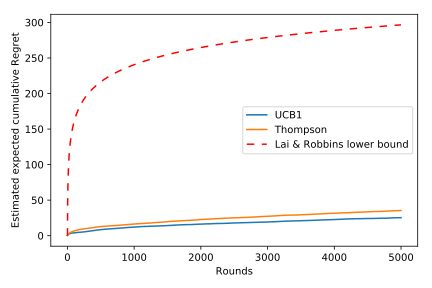
\includegraphics[width=\textwidth]{ex1_bernoulli_regret_2}
  %     \caption{Estimated expected cumulative regret for UCB1 and TS,
  %       and Lai-Robbins lower bound}\label{fig:ex1-bernoulli-arms-regret-2}
  %   \end{subfigure}
  %   \caption{Representation of the arms means and expected cumulative
  %     regret for the second chosen Bernoulli bandit}\label{fig:ex1-bernoulli-2}
  % \end{figure}
